\newpage
\section[Selecting mu rec and mu bwd]{Selecting $\mu_\text{rec}$ and $\mu_{\text{bwd}}$}
\label{sec:scaling-of-truncated-backpropigation}


\begin{figure}[h]
    \centering
    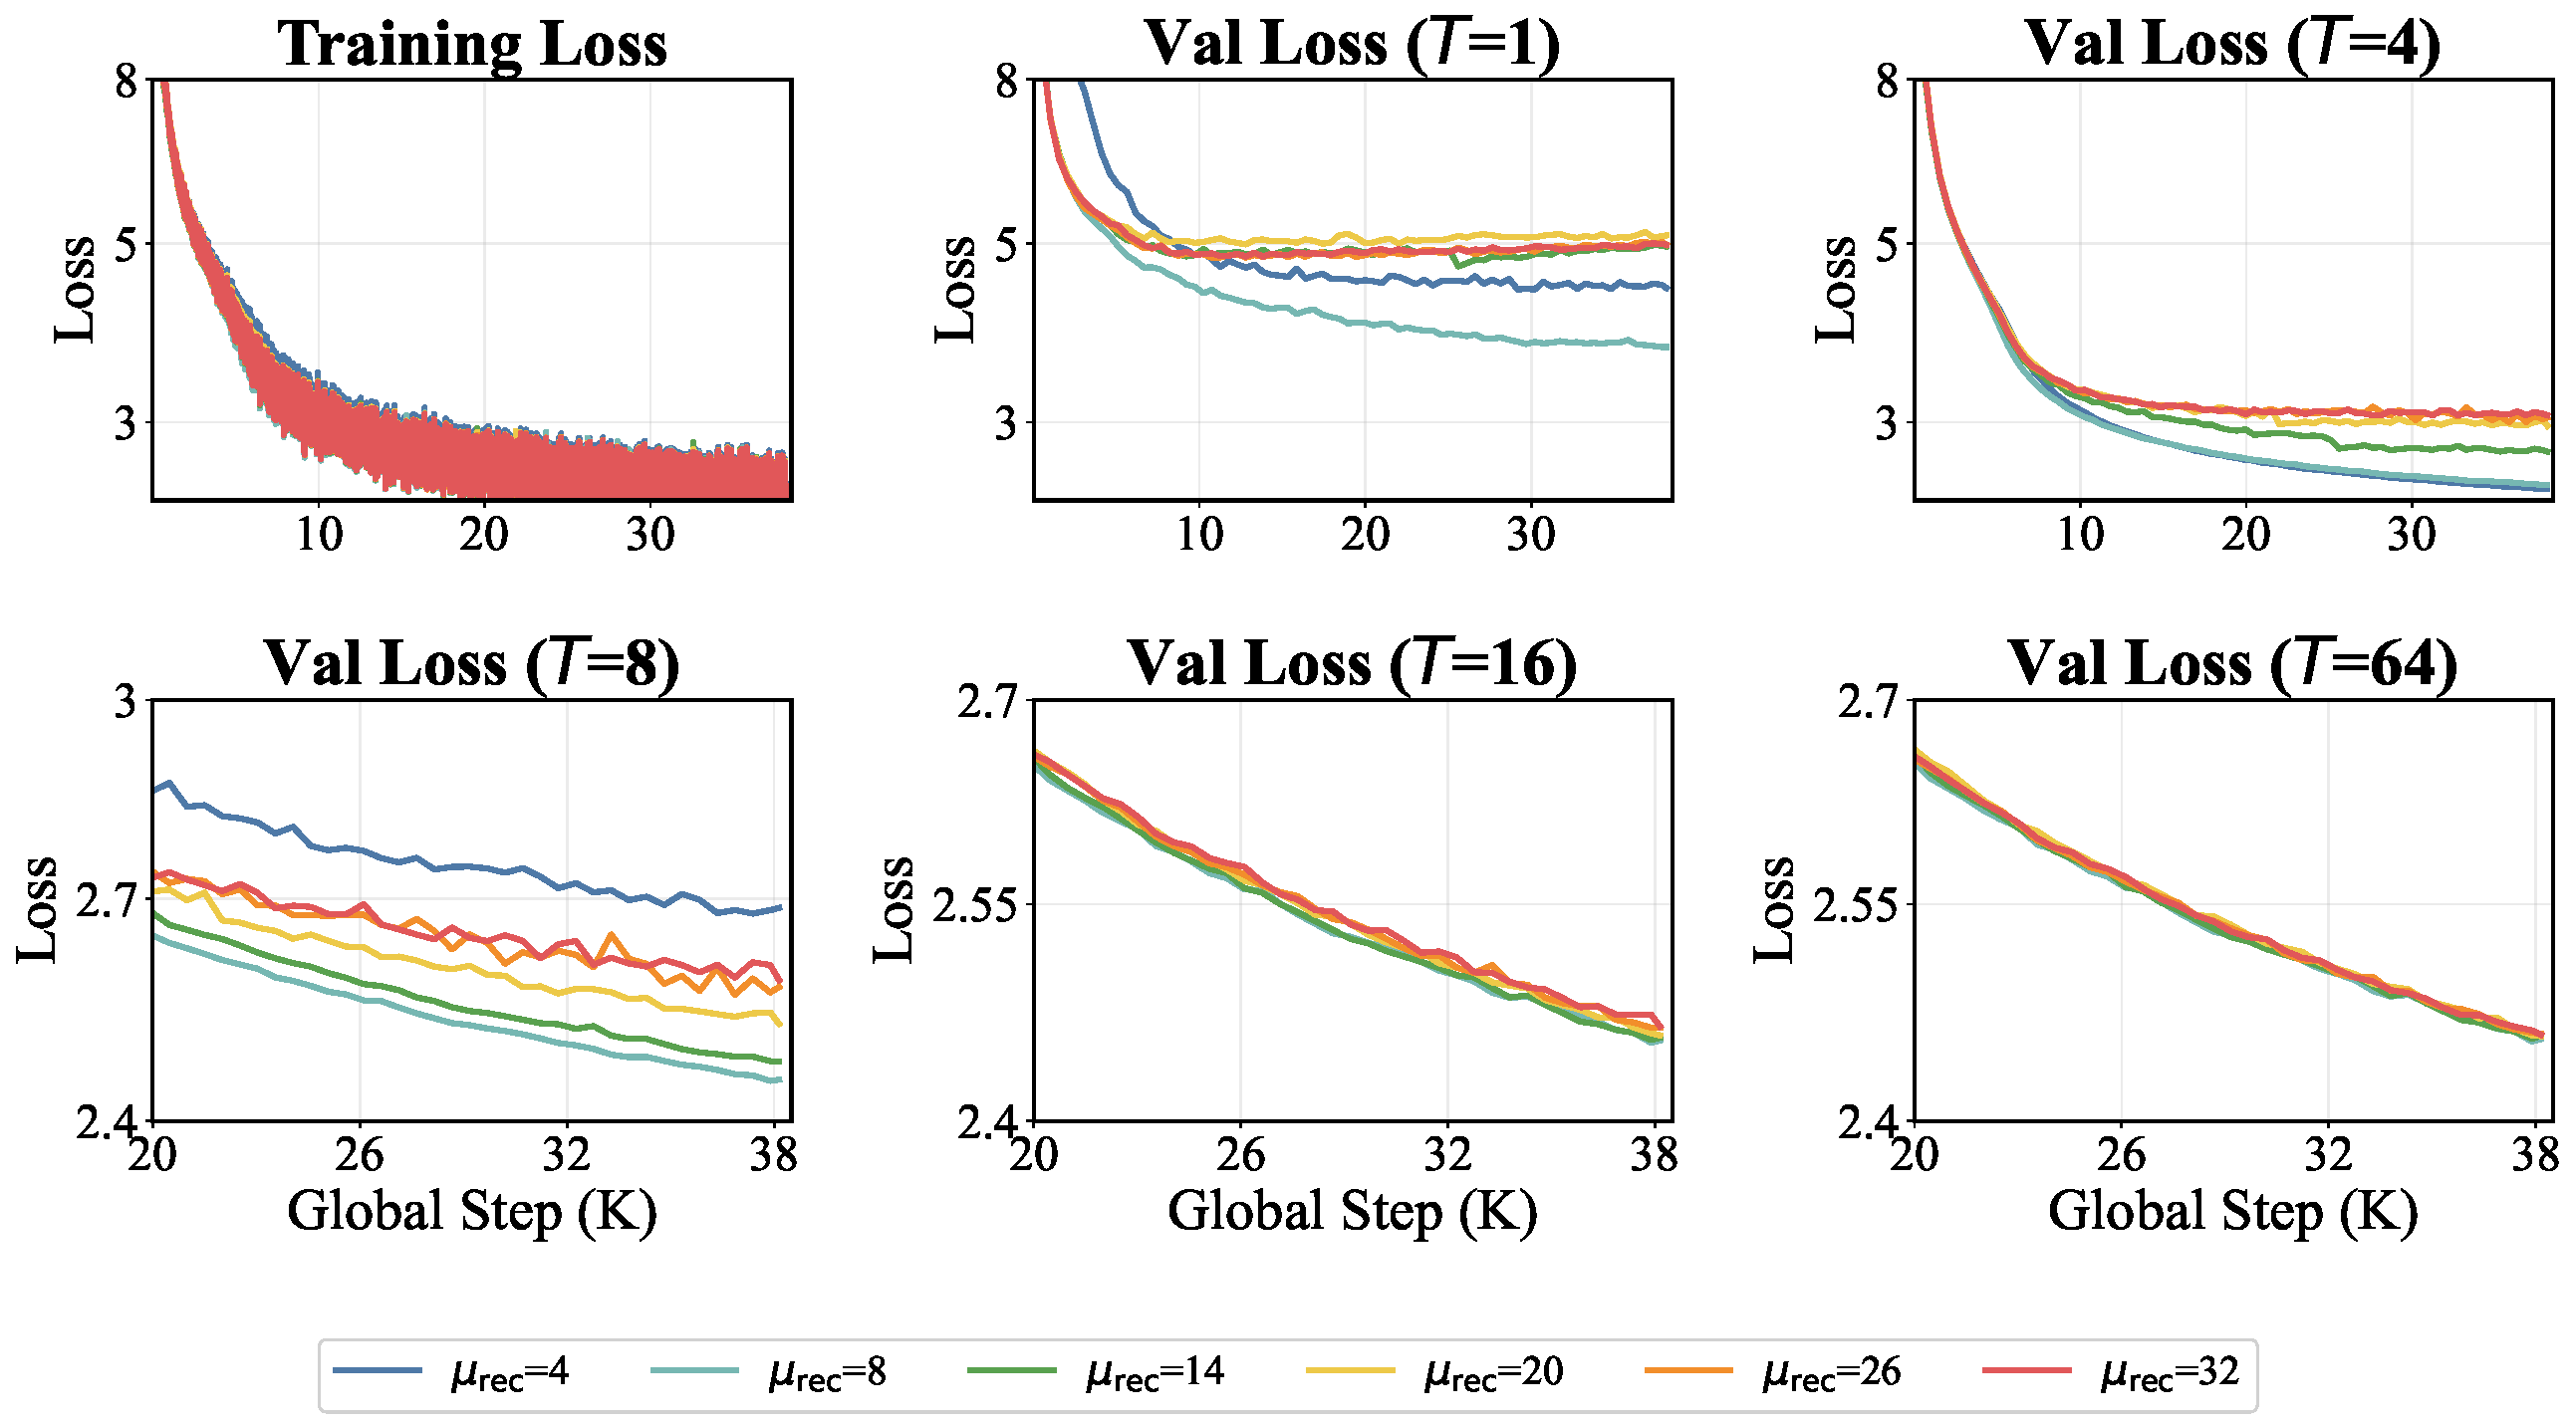
\includegraphics[width=\linewidth]{figures/appendix/mean_depth_loss_curves.pdf}
    \caption{Validation curves of six different recurrent depth models, pretrained on 10 billion tokens, with a fixed architecture and hyperparameters. Each model is pretrained with a fixed \meanbackward of 8 and varying \meanrecurrence in $[4,8,14,20,26,32]$. The key observation is that scaling up \meanrecurrence while keeping \meanbackward fixed results in models that perform worse than if just pretrained on \meanrecurrence of eight.}
    \label{fig:mean-recurrence-scaling}
\end{figure}

\begin{table}[h]
    \centering
    \begin{tabular}{ccccccc}
    \toprule
         & $\mu_{\text{rec}}=4$ & $\mu_{\text{rec}}=8$ & $\mu_{\text{rec}}=14$ & $\mu_{\text{rec}}=20$ & $\mu_{\text{rec}}=26$ & $\mu_{\text{rec}}=32$\\
         \midrule
         Val Loss & 2.477 & \textbf{2.453} & 2.456 & 2.457 & 2.458 & 2.458 \\
         Val Perplexity & 11.906 & \textbf{11.624} & 11.665 & 11.671 & 11.692 & 11.687 \\
         \bottomrule
    \end{tabular}
    \caption{Validation loss and perplexity for looped models trained with different \meanrecurrence and a fixed $\mu_{\text{bwd}}=4$. We use $T=\mu_{\text{rec}}$. Surprisingly, $\mu_{\text{rec}}=8$ performs the best.}
    \label{tab:mean-forward-results}
\end{table}

A natural question is what choice of \meanrecurrence and \meanbackward is appropriate for pretraining looped models. To answer this question, we conduct an experiment where we scale up \meanrecurrence, while keeping \meanbackward fixed. In our very initial experiments, we pretrained several small recurrent depth models \citep{geiping_scaling_2025} on 10 billion tokens, with a fixed $\mu_{\text{bwd}}=4$ and with $\mu_{\text{rec}} \in [4,8,14,20,26,32]$\footnote{Note that these experiments were run before the distribution mismatch fix discussed in \cref{sec:sampling-truncated-recurrence}. As the mismatch becomes more drastic as \meanrecurrence gets closer to \meanbackward, we expect the model pretrained with $\mu_{\text{rec}}=4$ to be performing sub-optimally.}. The results for each of these models on a held-out set of validation data can be observed in \cref{fig:mean-recurrence-scaling}. We additionally include \cref{tab:mean-forward-results}, which gives the validation loss of each model with $\mu_{\text{rec}} \in [4,8,14,20,26,32]$, where the recurrence that we use for each model at test-time is $T=\mu_{\text{rec}}$. 

The fascinating observation of \cref{fig:mean-recurrence-scaling} is that, contrary to our initial beliefs, models trained with additional \meanrecurrence beyond 8 perform worse at both lower and higher $r$ used at test-time, though more FLOPs were spent during pretraining. While it is a natural expectation that models trained with lower \meanrecurrence perform better than models with larger \meanrecurrence at low $T$, the fact that a \meanrecurrence of eight performs the best at higher $T$ (i.e., $T=16$ and $T=64$) is surprising. To determine if this is an inherent limitation of the capacity of looped models or an artifact of \meanbackward, we ran an additional experiment where we fixed $\mu_{rec}=20$ and instead varied $\mu_{\text{bwd}} \in [4,6,8,10,12]$, pretraining on 8.5 billion tokens for each model. We keep hyperparameters fixed. The results for each of these models on a held-out set of validation data can be visualized in \cref{fig:mean-backward-recurrence-scaling} and \cref{tab:mean-backward-results}.

\begin{figure}[h]
    \centering
    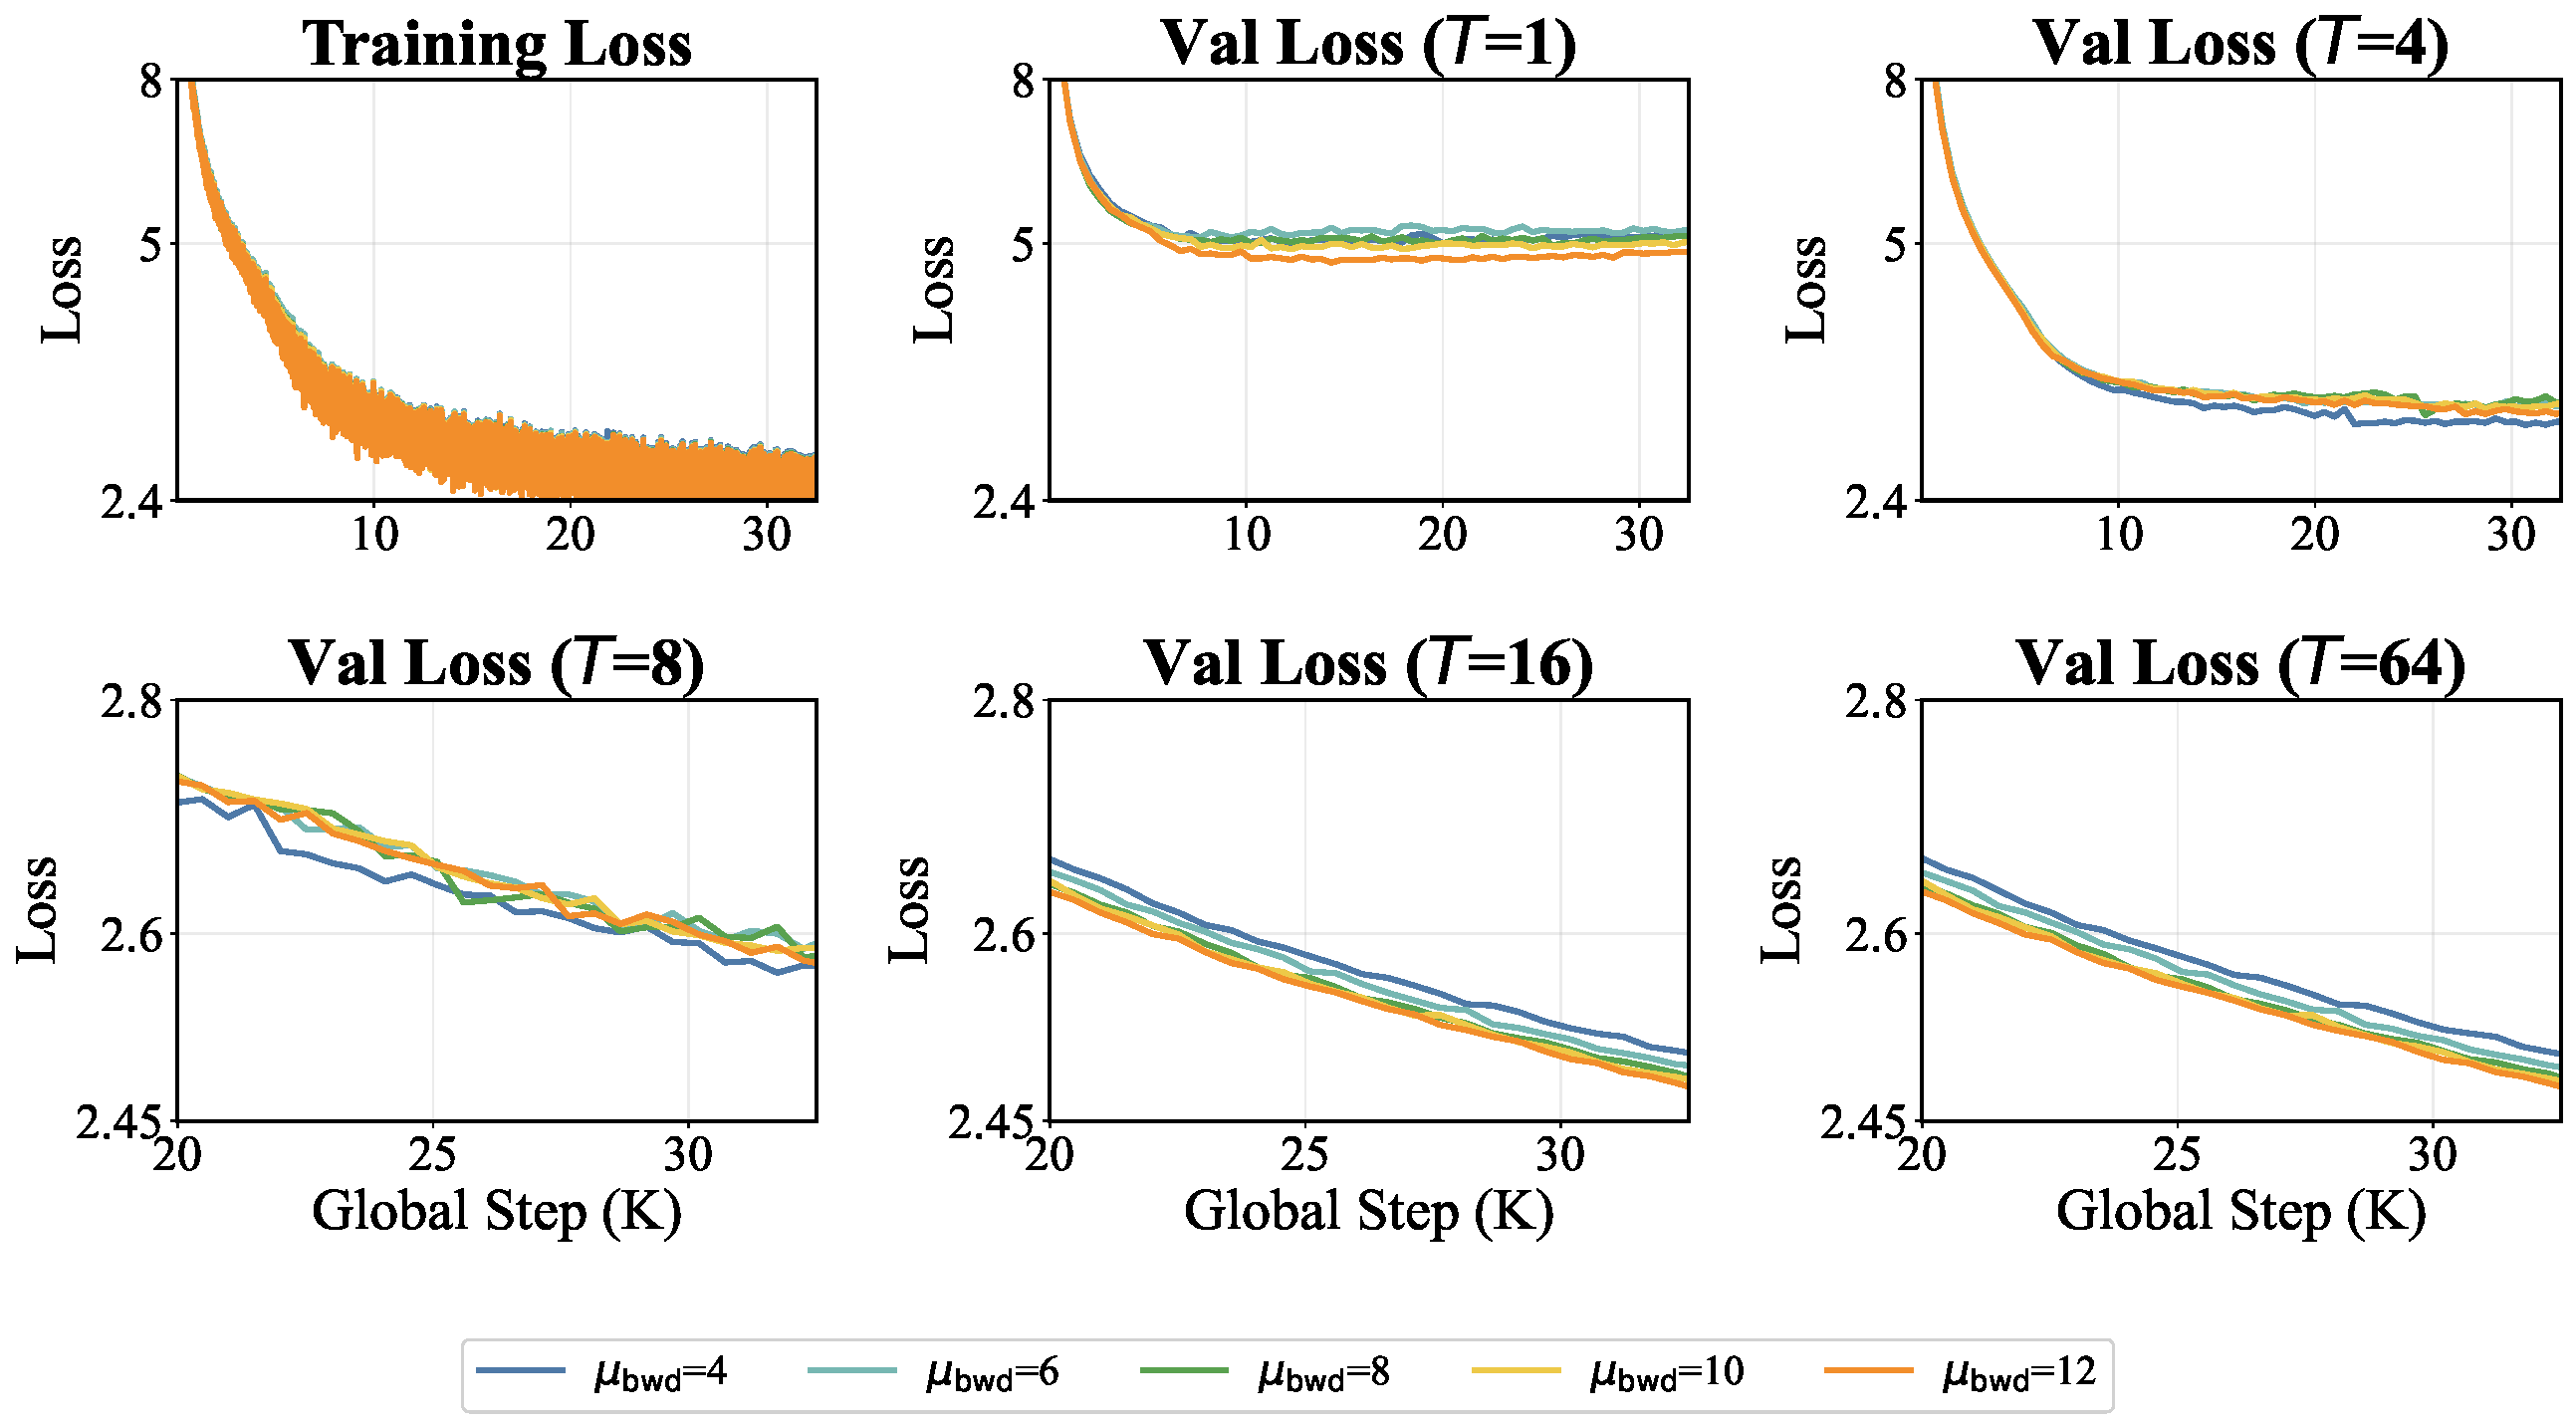
\includegraphics[width=\linewidth]{figures/appendix/mean_back_depth_loss_curves.pdf}
    \caption{Validation and training curves of looped models, pretrained on 8.5 billion tokens. Each model is trained with a fixed $\mu_{\text{rec}}=20$ and $\mu_{bwd} \in [4,6,8,10,12]$. Observe that scaling up \meanbackward improves validation performance at higher and lower recurrences monotonically for $T=1,16,64$.}
    \label{fig:mean-backward-recurrence-scaling}
\end{figure}

\begin{table}[h]
    \centering
    \begin{tabular}{cccccc}
    \toprule
         & $\mu_{\text{bwd}}=4$ & $\mu_{\text{bwd}}=6$ & $\mu_{\text{bwd}}=8$ & $\mu_{\text{bwd}}=10$ & $\mu_{\text{bwd}}=12$ \\
         \midrule
         Val Loss & 2.500 & 2.490 & 2.480 & 2.479 & \textbf{2.474} \\
         Val Perplexity & 12.09 & 12.06 & 11.94 & 11.93 & \textbf{11.86} \\
         \bottomrule
    \end{tabular}
    \caption{Validation loss and perplexity of looped models trained with variable \meanbackward, but fixed \meanrecurrence.}
    \label{tab:mean-backward-results}
\end{table}

While lower \meanbackward (i.e., $\mu_{\text{bwd}}=4,6,8$) appears to perform better with lower validation recurrences than higher \meanbackward, the validation loss using $T=16,64$ improves as \meanbackward increases. This implies that the capabilities of looped models utilizing deeper recurrences are heavily coupled with \meanbackward. However, it can be observed that increasing \meanbackward from ten to twelve has minimal impact on validation performance, at the cost of higher pretraining FLOPs. Using this insight, for our main training runs, we choose to use 
\begin{equation}
\mu_{\text{bwd}} = \lceil \frac{\mu_{\text{rec}}}{2} \rceil
\label{equation:mean-backward}
\end{equation}
We leave the exploration of FLOP optimal choices of \meanrecurrence and \meanbackward to future work.
